\documentclass[runningheads]{llncs}

\usepackage{amsmath,amssymb,amsfonts}
\usepackage{algorithm}
\usepackage{algpseudocode}
\usepackage{graphicx}
\usepackage{booktabs}
\usepackage{textcomp}
\usepackage{xcolor}
\usepackage[hidelinks]{hyperref}
\renewcommand\UrlFont{\color{blue}\rmfamily}

% Float placement: allow floats to share pages with text, which keeps the
% single-column layout from leaving half-empty pages around the wide tables.
\renewcommand{\topfraction}{0.92}
\renewcommand{\bottomfraction}{0.85}
\renewcommand{\textfraction}{0.06}
\renewcommand{\floatpagefraction}{0.85}
\setcounter{topnumber}{3}
\setcounter{bottomnumber}{2}
\setcounter{totalnumber}{4}


% Two-line table headers, used by tab_overall.tex and tab_null.tex
\newcommand{\hd}[2]{\begin{tabular}[b]{@{}r@{}}#1\\#2\end{tabular}}

\newcommand{\nABLADstatisticMAE}{0.547}
\newcommand{\nABLADstatisticNULL}{90.0}
\newcommand{\nABLGaussiannullMAE}{0.725}
\newcommand{\nABLGaussiannullNULL}{77.5}
\newcommand{\nABLnminfourzeroMAE}{1.066}
\newcommand{\nABLnminfourzeroNULL}{88.8}
\newcommand{\nABLnminonefiveMAE}{0.491}
\newcommand{\nABLnminonefiveNULL}{85.0}
\newcommand{\nABLnomultiplicitycorrMAE}{0.412}
\newcommand{\nABLnomultiplicitycorrNULL}{82.5}
\newcommand{\nABLproposedMAE}{0.381}
\newcommand{\nABLproposedNULL}{96.2}
\newcommand{\nALBEST}{6.91}
\newcommand{\nALBESTM}{HDBSCAN}
\newcommand{\nALBETTER}{14}
\newcommand{\nALCHI}{1653}
\newcommand{\nALNB}{1010}
\newcommand{\nALNS}{1}
\newcommand{\nALNSLIST}{HDBSCAN}
\newcommand{\nALP}{$<10^{-16}$}
\newcommand{\nALPOS}{2}
\newcommand{\nALRANK}{7.00}
\newcommand{\nALWORSE}{0}
\newcommand{\nALWORSELIST}{}
\newcommand{\nAUCPMED}{0.73}
\newcommand{\nAUCSEP}{0.80}
\newcommand{\nCANONELIST}{dip-means (100\%), CDK (94\%), G-means (52\%), HDBSCAN (51\%), MDL split/merge (50\%)}
\newcommand{\nCDKARI}{0.784}
\newcommand{\nCDKEX}{70.1}
\newcommand{\nCDKEXS}{63.5}
\newcommand{\nCDKKINIT}{15.1}
\newcommand{\nCDKMAE}{0.70}
\newcommand{\nCDKMAEabl}{0.381}
\newcommand{\nCDKNTEST}{37.3}
\newcommand{\nCDKNULL}{93.8}
\newcommand{\nCDKNULLabl}{96.2}
\newcommand{\nCDKREALARI}{0.207}
\newcommand{\nCDKREALMAE}{3.42}
\newcommand{\nCDKRNULL}{90.0}
\newcommand{\nCDKRNULLK}{1.1}
\newcommand{\nCDKTIME}{3.80}
\newcommand{\nCHT}{11.5}
\newcommand{\nCOV}{0.766}
\newcommand{\nCOVW}{1.5}
\newcommand{\nDIPSEPKfive}{4.6}
\newcommand{\nDIPSEPKten}{4.0}
\newcommand{\nDIPSEPKthree}{3.0}
\newcommand{\nDIPSEPKtwenty}{7.3}
\newcommand{\nDIPSEPKtwo}{2.0}
\newcommand{\nMULTDROP}{14}
\newcommand{\nNABL}{5}
\newcommand{\nNABLB}{320}
\newcommand{\nNBLOCK}{1010}
\newcommand{\nNCANONE}{5}
\newcommand{\nNCOLLAPSE}{63}
\newcommand{\nNMETH}{16}
\newcommand{\nNMETHM}{15}
\newcommand{\nNNULLB}{230}
\newcommand{\nNREALNULL}{7}
\newcommand{\nNREALSET}{15}
\newcommand{\nNROWS}{17170}
\newcommand{\nNSTRUCT}{780}
\newcommand{\nNSTRUCTCDK}{780}
\newcommand{\nNSYNSPEC}{43}
\newcommand{\nORCARI}{0.897}
\newcommand{\nPMEDCOL}{0.12}
\newcommand{\nPMEDOK}{0.14}
\newcommand{\nRATIOGAP}{8}
\newcommand{\nRATIOSIL}{21}
\newcommand{\nRNCalinskiHar}{2.9}
\newcommand{\nRNEXCalinskiHar}{0}
\newcommand{\nRNEXGapstatistic}{0}
\newcommand{\nRNEXGmeans}{29}
\newcommand{\nRNEXHDBSCAN}{29}
\newcommand{\nRNEXSilhouette}{0}
\newcommand{\nRNEXXmeans}{0}
\newcommand{\nRNEXdipmeans}{100}
\newcommand{\nRNGapstatistic}{3.3}
\newcommand{\nRNGmeans}{3.1}
\newcommand{\nRNHDBSCAN}{1.9}
\newcommand{\nRNSilhouette}{2.5}
\newcommand{\nRNXmeans}{10.3}
\newcommand{\nRNdipmeans}{1.0}
\newcommand{\nSEPCOLFLAG}{22}
\newcommand{\nSEPCOLUNFLAG}{3.0}
\newcommand{\nSEPDfifty}{0.11}
\newcommand{\nSEPDten}{0.11}
\newcommand{\nSEPDtwo}{0.15}
\newcommand{\nSEPEVCOL}{0.35}
\newcommand{\nSEPEVOK}{0.55}
\newcommand{\nSEPFLAGPCT}{27}
\newcommand{\nSEPKfive}{5.0}
\newcommand{\nSEPKten}{10.1}
\newcommand{\nSEPKthree}{3.0}
\newcommand{\nSEPKtwenty}{19.5}
\newcommand{\nSEPKtwo}{2.0}
\newcommand{\nSEPPREC}{22}
\newcommand{\nSEPREC}{73}
\newcommand{\nSEPTHR}{0.42}
\newcommand{\nSILU}{10.1}
\newcommand{\nSTBEST}{7.03}
\newcommand{\nSTBESTM}{Davies-Bouldin}
\newcommand{\nSTBETTER}{7}
\newcommand{\nSTCHI}{1597}
\newcommand{\nSTNB}{780}
\newcommand{\nSTNS}{1}
\newcommand{\nSTNSLIST}{GMM+ICL}
\newcommand{\nSTP}{$<10^{-16}$}
\newcommand{\nSTPOS}{9}
\newcommand{\nSTRANK}{8.35}
\newcommand{\nSTWORSE}{7}
\newcommand{\nSTWORSELIST}{Bisecting+Sil., Calinski-Har., Davies-Bouldin, Elbow (Kneedle), Gap statistic, HDBSCAN, Silhouette}


% Public repository for code and results (camera-ready, reviewer 4 item 6)
\newcommand{\repourl}{https://github.com/barunkrpaul/cdk-icadcml2027}

% ---------------------------------------------------------------------
% ICADCML 2027 reviews papers double-blind. Set \anontrue below to build
% the anonymous submission PDF, and \anonfalse for the camera-ready one.
% Nothing else in the file needs to change.
% ---------------------------------------------------------------------
\newif\ifanon
\anonfalse

\begin{document}

\title{Determining $k$ Without a Range: A Certified Divisive Test and What
Current Benchmarks Cannot Measure}

\titlerunning{Determining $k$ Without a Range}

\ifanon
  \author{Anonymous Author(s)}
  \authorrunning{Anonymous}
  \institute{Affiliation withheld for double-blind review}
\else
  \author{Barun Kr. Paul\inst{1,2} \and Kinsuk Giri\inst{1}}
  \authorrunning{B. Kr. Paul and K. Giri}
  \institute{National Institute of Technical Teachers' Training and Research
  (NITTTR) Kolkata, Salt Lake, Kolkata, West Bengal, India\\
  \email{kinsuk@nitttrkol.ac.in}
  \and
  Srikrishna College, Bagula, Nadia, West Bengal, India\\
  \email{barunkrpaul.cse@gmail.com}}
\fi

\maketitle

\begin{abstract}
Almost every published method for choosing $k$ in $K$-means is tested only on
datasets that already contain clusters, which hides an important difference. A
method that scores a criterion over a user-supplied range
$k \in \{2,\dots,k_{\max}\}$ can never return the answer $k=1$, so on such a
benchmark it looks the same as a method that really reads $k$ from the data.
The difference is made measurable here by adding structureless datasets to the
protocol, including real single-class extracts and not only synthetic noise.
We also present CDK, a divisive procedure with no candidate range at all. CDK
over-partitions the data by repeated bisection, fixes a family of candidate
merges on the fragments, tests every candidate with a normalised energy
statistic calibrated by Monte Carlo against a matched null model, and returns
the connected components that survive a multiplicity-corrected threshold. Over
\nNBLOCK{} blocks and \nNMETH{} methods the choice of benchmark decides the
conclusion. On blocks that contain clusters CDK ranks \nSTPOS{} of \nNMETH{}
and \nSTWORSE{} competitors beat it, while adding the structureless blocks
moves it to \nALPOS{} with no method beating it. CDK returns $k=1$ on
\nCDKNULL\% of synthetic structureless blocks and \nCDKRNULL\% of real
single-class blocks, where every range-based method scores zero by
construction.

\keywords{Clustering \and Number of clusters \and $K$-means \and Hypothesis
testing \and Energy distance \and Multiple testing \and Cluster validity}
\end{abstract}

% =====================================================================
\section{Introduction}

$K$-means needs $k$. The literature on supplying it is large and still
growing, and most of it follows one pattern. A criterion is defined, evaluated
at every $k$ in a range the user supplies, and the $k$ that optimises it is
reported. Silhouette \cite{rousseeuw1987silhouettes}, Calinski-Harabasz
\cite{calinski1974dendrite}, Davies-Bouldin \cite{davies1979cluster}, the jump
statistic \cite{sugar2003finding} and the gap statistic
\cite{tibshirani2001gap} all work this way, and so do the many indices
proposed since.

The user-supplied range is usually treated as a harmless implementation
detail. It is not. A criterion evaluated on $\{2,\dots,k_{\max}\}$ has no way
to express the answer $k=1$, and $k=1$ is correct whenever the data carry no
cluster structure. Such a method does not determine $k$. It ranks the
candidates it was given, with the same confidence on uniform noise as on ten
clean Gaussians, so $k$ has only been replaced by $k_{\max}$ and by the
assumption that at least two clusters exist. This would be a small point if
benchmarks tested it. We are not aware of any published comparison of
$k$-selection methods that includes even one dataset with $k^\star = 1$, so on
the usual benchmark the two kinds of method produce the same kind of table.

Three contributions are made here. The first is about evaluation, viz.\
structureless data are added to the protocol as synthetic nulls of four kinds
in two dimensionalities and as \nNREALNULL{} single-class extracts from
standard real datasets, the latter being the closest thing the usual
repositories offer to real data known to come from one labelled population.
The second is an algorithm. CDK, short for Certified Divisive $k$, determines
$k$ with no candidate range and no $k_{\max}$, by over-partitioning the data,
fixing a candidate merge family, testing each candidate with a nonparametric
two-sample statistic calibrated by Monte Carlo, and applying one multiplicity
correction over that family. The third is a demonstration that the omission is
not small, since the same \nNMETH{} methods, run on the same data, invert
their ranking once the structureless blocks are included. The limitations of
CDK are reported alongside, in Sections~\ref{sec:results}
and~\ref{sec:limits}.

% =====================================================================
\section{Automatic Versus Range-Restricted Methods}
\label{sec:auto}

Four behaviours are distinguished here that the literature usually reports
under the single heading of automatic $k$ selection. In \textbf{AUTO} methods
the value of $k$ is determined by the data over an unbounded range and $k=1$
can be returned; examples in our pool are CDK, dip-means
\cite{kalogeratos2012dipmeans}, G-means \cite{hamerly2003gmeans} and HDBSCAN
\cite{campello2013hdbscan}. In \textbf{RANGE} methods a criterion is optimised
over a user-supplied set $\{2,\dots,k_{\max}\}$, so the output is a ranking of
the supplied candidates and $k=1$ is not among them; all classical validity
indices fall here. In \textbf{SUBSTITUTED} methods $k$ is removed but another
free parameter carrying the same role is introduced, such as a penalty weight,
a bandwidth or a density radius, so the parameter has moved rather than
vanished. In \textbf{NOT-AUTO} methods $k$ remains an explicit input.

A RANGE method applied to data with no clusters returns a confident partition
of noise with no signal that anything is wrong, and a benchmark with no
$k^\star=1$ case cannot measure this difference.

% =====================================================================
\section{Related Work}
\label{sec:related}

\noindent\textbf{Split tests inside $K$-means.} X-means
\cite{pelleg2000xmeans} splits a centre when the two-centre model improves
BIC, G-means \cite{hamerly2003gmeans} splits when an Anderson-Darling test
rejects Gaussianity of a projection, and PG-means \cite{feng2006pgmeans}
increases $k$ until projected Kolmogorov-Smirnov tests stop rejecting the
fitted mixture. Dip-means \cite{kalogeratos2012dipmeans} and Skinny-dip
\cite{maurus2016skinnydip} use Hartigan's dip test. All grow $k$ from the top
down, and none applies any correction across the many tests it performs.

\medskip\noindent\textbf{Simulated nulls.} SigClust \cite{liu2008sigclust}
tests whether a two-means split is real by comparing a within-cluster
sum-of-squares ratio against Monte Carlo draws from a fitted single-Gaussian
null, and its hierarchical extension \cite{kimes2017shc} tests every node of a
dendrogram against the same null under a sequential family-wise rule. No novelty is
claimed here for calibrating a partition test against a simulated null. The gap
statistic \cite{tibshirani2001gap} introduced the uniform reference
distribution, so the reference geometry used by CDK is also established.

\medskip\noindent\textbf{Over-partition and then merge.} This architecture is
not new either. RSEC \cite{risso2018rsec} over-clusters with an ensemble and
decides each merge from the proportion of differentially expressed genes under
false discovery rate control. UniForCE \cite{vardakas2026uniforce}
over-clusters with $K$-means, tests pairs of fragments for unimodality with a
dip test on the projection onto the line joining their centroids, and
assembles a spanning forest from the accepted pairs, which makes it the
nearest neighbour of CDK here.

\medskip\noindent\textbf{Contribution relative to prior work.} Three narrow
claims are made, and no wider one. (i) The test statistic is a normalised energy distance
\cite{szekely2013energy} between the two sides of a candidate merge, and no
prior work could be found that uses energy distance as the decision statistic
for choosing $k$. (ii) Each reference draw is bisected by the same randomised
two-means mechanism that produced the observed bisection, so the two
statistics come from a matched procedure. (iii) The candidate family is fixed
before any test is run and corrected once with a closed-form threshold, rather
than discovered greedily as in UniForCE, which applies no correction, or
tested sequentially down a dendrogram as in \cite{kimes2017shc}. Whether these
refinements justify a new method is tested in the experiments.

% =====================================================================
\section{The CDK Procedure}
\label{sec:method}

\subsection{Over-partition and Candidate Family}

CDK first bisects the data recursively with two-means. Any node holding at
least $2n_{\min}$ points is split, and the recursion stops otherwise. The
parameter $n_{\min}$ is a resolution floor and not a cluster count, since it
says how small a group must be before the procedure declines to look inside
it. The result is $k_{\text{init}}$ leaves, deliberately many more than
$k^\star$, with a mean of $k_{\text{init}} = \nCDKKINIT{}$ in our experiments.
Section~\ref{sec:corrections} says why the procedure over-partitions rather
than testing from the top down. Each leaf is then joined to its
$n_{\text{nb}}$ nearest leaves by centroid distance, producing a fixed family
$E$ of $m = |E|$ candidate merges. The family follows from the geometry of the
leaves and is fixed before any test is run, which is what makes a single
multiplicity correction over it legitimate.

\subsection{The Merge Test}

For a candidate merge of leaves $A$ and $B$, the null hypothesis is that
$A \cup B$ is one population. The normalised energy statistic is used, viz.
\begin{equation}
T(A,B) = \frac{2\,\overline{d}(A,B) - \overline{d}(A,A) - \overline{d}(B,B)}
              {\overline{d}(A \cup B)},
\end{equation}
where $\overline{d}(\cdot,\cdot)$ denotes a mean pairwise Euclidean distance
between or within the indicated sets. The numerator is the energy distance
\cite{szekely2013energy}, which is zero if and only if the two samples come
from the same distribution. The denominator makes the statistic invariant to
the scale of the parent, so a threshold learned at one node transfers to
another.

The reference distribution is obtained by Monte Carlo. $R$ synthetic datasets
of the same size as $A \cup B$ are drawn from a matched null model, namely a
uniform distribution over a box aligned to the principal axes of the parent.
Each draw is bisected by the same randomised two-means mechanism used on the
observed data, and $T$ is computed on the result, giving
$p = (1 + \#\{r : T_r \ge T_{\text{obs}}\})/(1 + R)$. If the observed
partition were inherited from an ancestor while the reference partition was
drawn afresh, the two statistics would not be comparable and the test would
over-reject, which was observed before the mechanisms were matched.

\subsection{Assembly Under Multiplicity Control}

Rejecting an edge asserts that its two leaves are separate groups, so what
must be controlled is the number of spurious separations across the family. A
merge is accepted when
\begin{equation}
p_e > \alpha_m, \qquad
\alpha_m = \max\!\left(\frac{q}{m},\ \frac{2}{R+1}\right),
\end{equation}
which is a Bonferroni-style threshold floored at the Monte Carlo resolution,
since no p-value below $1/(R+1)$ can be observed. The returned clusters are
the connected components of the graph of accepted merges, and $\hat k$ is
their number, bounded only by $k_{\text{init}}$. There is no candidate range
anywhere in the procedure, which Algorithm~\ref{alg:cdk} states in full.

\medskip\noindent\textbf{Scope of the term ``certified''.} The word refers to
one property and no more. If every candidate merge in $E$ joins two pieces of
one population, the Bonferroni inequality bounds the probability that any of
them is rejected by $m\alpha_m$, so a separation reported by CDK rests on a
test whose family-wise error is bounded in this sense. The bound holds only to
the extent that the matched reference describes the data under the null. It is
conservative, because the edge tests are dependent. It equals $q$ only when
$R+1 \ge 2m/q$; otherwise the Monte Carlo floor binds and the bound is
$2m/(R+1)$, which is weaker. It also assumes that the candidate graph connects
the leaves of each true cluster, since two leaves joined by no candidate edge
are separated without any test. CDK therefore does not provide a confidence
statement about $k^\star$ itself.

\begin{algorithm}[!htbp]
\caption{CDK}
\label{alg:cdk}
\begin{algorithmic}[1]
\Require $X$, level $q$, draws $R$, floor $n_{\min}$, degree $n_{\text{nb}}$
\State $L \gets$ recursive two-means bisection of $X$ to floor $n_{\min}$
\State $E \gets$ each leaf joined to its $n_{\text{nb}}$ nearest leaves
\State $m \gets |E|$; \ $\alpha_m \gets \max(q/m,\ 2/(R+1))$
\ForAll{$(A,B) \in E$}
  \State draw the observed bisection of $A \cup B$ by mechanism $\mathcal{M}$;
         $T_{\text{obs}} \gets T(A,B)$
  \For{$r = 1 \dots R$}
    \State $Z_r \sim$ null model matched to $A \cup B$; bisect $Z_r$ by
           $\mathcal{M}$; get $T_r$
    \State \textbf{break} if the outcome of the test is already determined
  \EndFor
  \State $p_e \gets (1 + \#\{T_r \ge T_{\text{obs}}\}) / (1 + R)$
\EndFor
\State $\hat k \gets$ number of connected components of
       $\{e \in E : p_e > \alpha_m\}$
\State \Return $\hat k$, labels, $\{p_e\}$, $\mathrm{median}_e\, p_e$
\end{algorithmic}
\end{algorithm}

The cost is $m R$ two-means fits on subsampled unions rather than on the full
data, and it does not depend on any $k_{\max}$. A direct two-means
replaces a general-purpose $K$-means call, which reduced the time per dataset
about six-fold, and a test is abandoned once $(1 + \text{hits})/(1 + R)$ has
passed $\alpha_m$.

% =====================================================================
\section{Design Revisions Made During Development}
\label{sec:corrections}

\noindent\textbf{Calibration by relabelling.} The original intention was to
calibrate the test against random relabellings of the points of the parent
node, which would have given a distribution-free null. A relabelling leaves the
point set unchanged as a multiset in $\mathbb{R}^d$, so a permutation-invariant
procedure such as $K$-means returns the same bisection and statistic on every
relabelled copy, and every p-value equals one. A null model is therefore
unavoidable. What remains free of distributional assumptions is the statistic
and not the reference, and CDK is described accordingly as a nonparametric
statistic with a model-based reference.

\medskip\noindent\textbf{Top-down testing.} Testing the root split first and
recursing returned $\hat k = 1$ on twenty separated clusters, because two
mixtures of about ten clusters each are not distinguishable by the statistic.
Over-partitioning first avoids this.

\medskip\noindent\textbf{Greedy sequential merging.} An intermediate version
merged greedily and stopped at the first non-rejection. With a mean of
\nCDKNTEST{} tests per dataset at level $0.05$ the probability of at least one
spurious rejection is $1 - 0.95^{\nCDKNTEST{}} \approx 0.86$, and $\hat k$ ran
between 21 and 41 on structureless data. The fixed family with a corrected
threshold replaced it.

% =====================================================================
\section{Experimental Protocol}
\label{sec:proto}

\noindent\textbf{Data.} \nNSYNSPEC{} synthetic specifications and
\nNREALSET{} real datasets give \nNBLOCK{} dataset and replicate blocks, of
which \nNSTRUCT{} have $k^\star > 1$ and \nNNULLB{} have $k^\star = 1$. The
synthetic families are well-separated blobs with
$k^\star \in \{2,3,5,10,20\}$ and $d \in \{2,10,50\}$, overlapping blobs at
four separations, unbalanced cluster sizes at three ratios, unequal variances,
elongated clusters at two condition numbers, non-Gaussian components ($t_3$,
uniform, mixed, skewed), uniform contamination at three levels, nested
hierarchical structure, and structureless data of four kinds (Gaussian,
uniform, $t_3$, anisotropic) in two dimensionalities. Of the real datasets,
eight are labelled, viz.\ Iris, Wine, Breast cancer, Digits, a 700-point
subsample of Digits, two Digits subsets, and a ten-component PCA projection of
Digits. The remaining \nNREALNULL{} are single-class extracts, each holding
all samples carrying one label from one of these datasets. They do not
guarantee unimodality, since a labelled class can carry substructure such as
handwriting style, so they are reported separately and read as a directional
signal.

\medskip\noindent\textbf{Competitors.} There are \nNMETH{} methods including
CDK. The range-based ones are Silhouette, Calinski-Harabasz, Davies-Bouldin,
the elbow by Kneedle \cite{satopaa2011kneedle}, the jump statistic, the gap
statistic, GMM with BIC \cite{schwarz1978estimating}, GMM with ICL
\cite{biernacki2000icl}, and bisecting $K$-means with a Silhouette stop. Each
searches $k \in \{\max(2, k^\star-5), \dots, \max(12, k^\star+5)\}$ with ten
restarts, a range centred on the truth and therefore generous to them. The
rest are X-means, G-means, dip-means, ISODATA, an MDL split and merge rule,
and HDBSCAN. An oracle running $K$-means at the true $k$ reaches
$\mathrm{ARI} = \nORCARI{}$ on the structured blocks, which bounds what any
correct $\hat k$ can achieve.

\medskip\noindent\textbf{Metrics and tests.} Absolute error
$|\hat k - k^\star|$, exact recovery rate, and ARI \cite{hubert1985comparing}
with contamination points excluded. For significance a Friedman test is used,
followed by pairwise Wilcoxon signed-rank tests against CDK with Holm
adjustment. The Nemenyi post-hoc test is avoided, because its mean-rank
statistic depends on which other methods happen to be in the pool
\cite{benavoli2016posthoc,demsar2006statistical}.

% =====================================================================
\section{Results}
\label{sec:results}

\subsection{The Benchmark Decides the Conclusion}
\label{sec:inversion}

Every method was run twice, differing only in which blocks enter the
comparison, and Table~\ref{tab:inversion} gives the result.

\begin{table}[!htbp]\centering
\caption{The same \nNMETH{} methods, the same runs, two benchmarks. The upper
row uses only blocks that contain clusters, as published comparisons do; the
lower row adds the structureless blocks. Counts come from Holm-adjusted
pairwise Wilcoxon signed-rank tests against CDK.}
\label{tab:inversion}
\begin{tabular}{lrrrr}
\toprule
Benchmark & blocks & CDK rank & beaten by & beats \\ \midrule
clusters only ($k^\star>1$) & \nSTNB{} & \nSTRANK{} (\nSTPOS/\nNMETH) &
  \nSTWORSE{} & \nSTBETTER{} \\
all blocks & \nALNB{} & \nALRANK{} (\nALPOS/\nNMETH) &
  \nALWORSE{} & \nALBETTER{} \\
\bottomrule
\end{tabular}
\end{table}

On the clusters-only benchmark CDK places \nSTPOS{} of \nNMETH{}, with
\nSTBESTM{} first at \nSTBEST{}, and seven methods beat it significantly,
viz.\ \nSTWORSELIST{}. Judged on this table alone, CDK would be an unremarkable method. Adding the
structureless blocks reverses this.
CDK moves to rank \nALRANK{}, place \nALPOS{} of \nNMETH{}, beating
\nALBETTER{} of the \nNMETHM{} others significantly, with no method beating it
and only \nALNSLIST{} not separated from it. No hyperparameter was retuned, no
dataset was replaced, and the runs are identical. The ordering
inverted because one family of datasets was restored, and that family is the
one on which the AUTO and RANGE behaviours of Section~\ref{sec:auto} differ.
This is the main empirical result, and it would hold for any AUTO method. Figure~\ref{fig:inversion} shows the same effect
for every method at once, while Table~\ref{tab:overall} gives the per-method
detail.

\begin{figure}[!htbp]
\centering
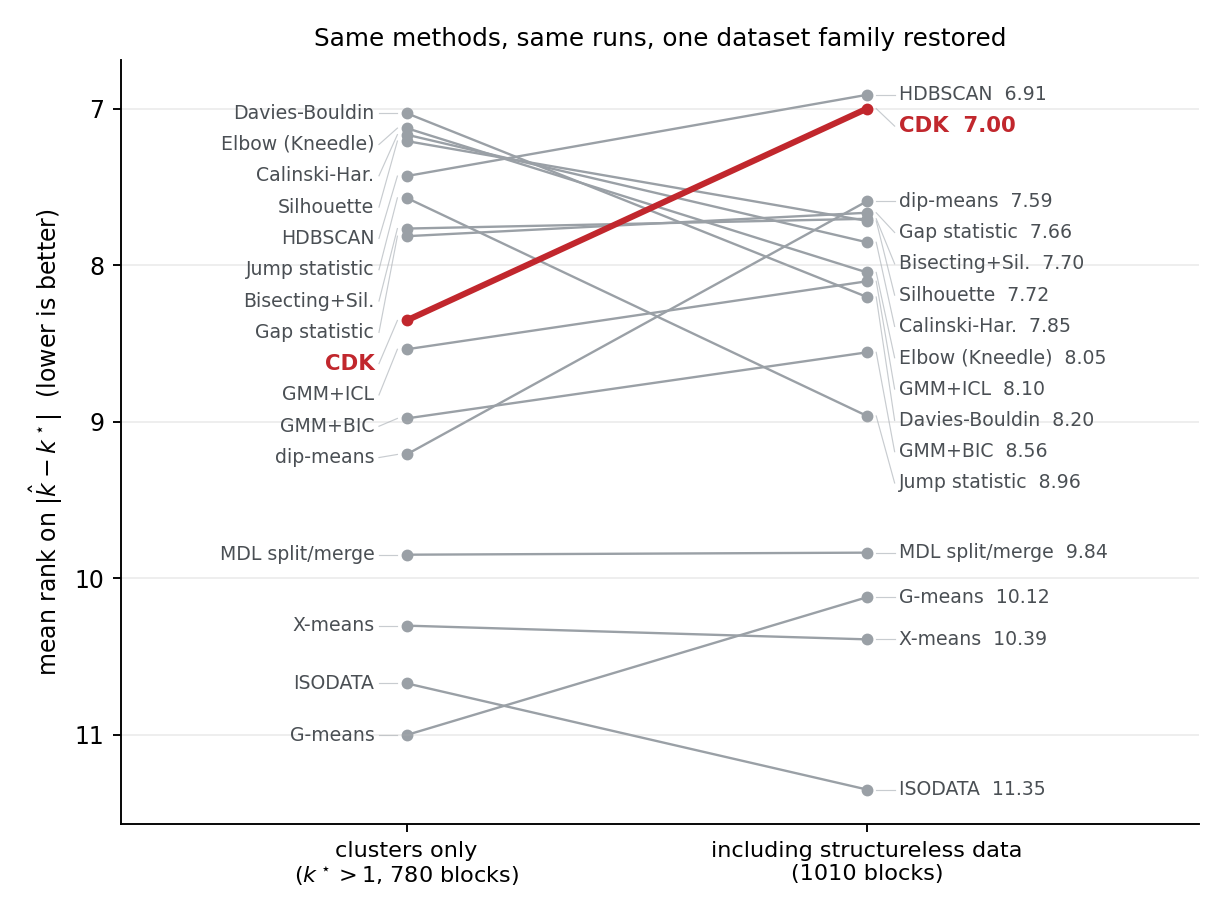
\includegraphics[width=0.46\textwidth]{figs/fig0_inversion.png}
\caption{Mean rank of every method under the two benchmarks. Only the set of
blocks entering the comparison differs.}
\label{fig:inversion}
\end{figure}

\begin{table}[!htbp]\centering
\caption{Headline results over all \nNBLOCK{} blocks of the full protocol, sorted by mean absolute error in $k$. ``struct.'' restricts to $k^\star>1$, ``real 1-cl.'' to the single-class real extracts.}
\label{tab:overall}
\footnotesize
\setlength{\tabcolsep}{4.5pt}
\renewcommand{\arraystretch}{0.85}
\resizebox{\textwidth}{!}{%
\begin{tabular}{lrrrrrrrr}
\toprule
Method & \hd{mean}{$|\hat k-k^\star|$} & \hd{exact}{all (\%)} & \hd{exact}{struct.\ (\%)} &
\hd{syn.\ null}{$\hat k{=}1$ (\%)} & \hd{real 1-cl.}{$\hat k{=}1$ (\%)} &
\hd{ARI}{all} & \hd{ARI}{struct.} & \hd{time}{(s)} \\ \midrule
\textbf{CDK} & 0.70 & 70.1 & 63.5 & 94 & 90 & 0.816 & 0.784 & 3.80 \\
HDBSCAN & 0.75 & 63.5 & 69.2 & 51 & 29 & 0.730 & 0.816 & 0.01 \\
Bisecting+Sil. & 0.92 & 53.8 & 69.6 & 0 & 0 & 0.651 & 0.843 & 0.13 \\
Gap statistic & 0.93 & 53.4 & 69.1 & 0 & 0 & 0.645 & 0.835 & 0.50 \\
GMM+ICL & 1.12 & 45.6 & 59.1 & 0 & 0 & 0.640 & 0.829 & 0.41 \\
GMM+BIC & 1.37 & 42.0 & 54.4 & 0 & 0 & 0.636 & 0.824 & 0.39 \\
Silhouette & 1.39 & 60.7 & 78.6 & 0 & 0 & 0.683 & 0.884 & 0.18 \\
Calinski-Har. & 1.41 & 61.3 & 79.4 & 0 & 0 & 0.668 & 0.864 & 0.12 \\
Elbow (Kneedle) & 1.43 & 58.5 & 75.8 & 0 & 0 & 0.638 & 0.826 & 0.12 \\
dip-means & 1.85 & 71.2 & 62.7 & 100 & 100 & 0.747 & 0.672 & 0.06 \\
Davies-Bouldin & 2.03 & 63.0 & 81.5 & 0 & 0 & 0.682 & 0.884 & 0.14 \\
G-means & 2.38 & 36.2 & 33.6 & 52 & 29 & 0.720 & 0.800 & 0.03 \\
X-means & 2.70 & 37.0 & 47.9 & 0 & 0 & 0.631 & 0.817 & 0.04 \\
Jump statistic & 2.95 & 62.3 & 80.6 & 0 & 0 & 0.669 & 0.866 & 0.12 \\
ISODATA & 3.88 & 29.1 & 37.7 & 0 & 0 & 0.580 & 0.750 & 0.02 \\
MDL split/merge & 4.33 & 54.6 & 59.1 & 50 & 14 & 0.708 & 0.802 & 0.14 \\
\bottomrule
\end{tabular}}
\end{table}


\subsection{Structureless Data}

Table~\ref{tab:null} is where the methods separate. On the synthetic nulls CDK
returns $\hat k = 1$ in \nCDKNULL\% of blocks, and on the real single-class
extracts in \nCDKRNULL\% of blocks, while every range-based method scores
zero. Silhouette reports a
mean of \nSILU{} clusters in ten-dimensional uniform noise and
Calinski-Harabasz reports \nCHT{} in bivariate $t_3$ noise, and these large
errors stay invisible on any benchmark that omits $k^\star = 1$.

\begin{table}[!htbp]\centering
\caption{Mean $\hat k$ on data with no cluster structure. The last column averages the single-class real extracts. The correct answer everywhere is 1.}
\label{tab:null}
\footnotesize
\setlength{\tabcolsep}{4pt}
\renewcommand{\arraystretch}{0.85}
\resizebox{\textwidth}{!}{%
\begin{tabular}{lrrrrrrrrr}
\toprule
Method & \hd{aniso}{$d$10} & \hd{aniso}{$d$2} & \hd{gauss}{$d$10} & \hd{gauss}{$d$2} &
\hd{$t_3$}{$d$10} & \hd{$t_3$}{$d$2} & \hd{unif}{$d$10} & \hd{unif}{$d$2} &
\hd{real}{1-cl.} \\ \midrule
\textbf{CDK} & 1.0 & 1.2 & 1.0 & 1.0 & 1.0 & 1.4 & 1.0 & 1.0 & 1.1 \\
HDBSCAN & 1.1 & 2.6 & 1.0 & 2.1 & 1.0 & 2.4 & 1.0 & 4.5 & 1.9 \\
Bisecting+Sil. & 2.0 & 2.0 & 2.0 & 2.4 & 2.1 & 7.2 & 2.0 & 4.0 & 2.0 \\
Gap statistic & 2.1 & 2.0 & 2.0 & 2.1 & 2.0 & 2.0 & 2.0 & 2.4 & 3.3 \\
GMM+ICL & 2.0 & 2.4 & 2.0 & 2.0 & 2.2 & 2.0 & 2.0 & 2.0 & 2.1 \\
GMM+BIC & 2.0 & 2.0 & 2.0 & 2.0 & 2.5 & 2.6 & 2.0 & 4.2 & 2.1 \\
Silhouette & 2.0 & 2.0 & 8.7 & 7.1 & 6.4 & 7.3 & 10.1 & 4.3 & 2.5 \\
Calinski-Har. & 2.0 & 7.5 & 2.0 & 6.8 & 2.2 & 11.5 & 2.0 & 9.8 & 2.9 \\
Elbow (Kneedle) & 5.2 & 4.9 & 5.9 & 5.3 & 5.8 & 5.6 & 5.8 & 4.0 & 5.1 \\
dip-means & 1.0 & 1.0 & 1.0 & 1.0 & 1.0 & 1.0 & 1.0 & 1.0 & 1.0 \\
Davies-Bouldin & 6.4 & 2.9 & 11.8 & 10.1 & 10.0 & 9.4 & 11.6 & 7.8 & 5.7 \\
G-means & 1.0 & 1.0 & 1.0 & 1.0 & 7.5 & 9.4 & 3.0 & 6.7 & 3.1 \\
X-means & 7.8 & 10.6 & 2.0 & 2.0 & 2.5 & 2.3 & 2.0 & 4.0 & 10.3 \\
Jump statistic & 11.4 & 6.0 & 10.6 & 6.5 & 11.6 & 10.1 & 10.9 & 6.0 & 11.8 \\
ISODATA & 11.7 & 7.0 & 12.0 & 7.1 & 11.1 & 7.8 & 12.0 & 7.0 & 9.6 \\
MDL split/merge & 17.0 & 7.3 & 1.0 & 1.0 & 17.0 & 3.9 & 1.0 & 1.0 & 14.0 \\
\bottomrule
\end{tabular}}
\end{table}


The comparison is asymmetric by construction, and these methods answer a
different question. Only
\nNCANONE{} of the \nNMETH{} methods returned $k=1$ anywhere in the study,
viz.\ \nCANONELIST. Among those, dip-means attains a perfect null score at the
cost of severe under-splitting elsewhere, recovering a mean of \nDIPSEPKten{} against
$k^\star = 10$ where CDK recovers \nSEPKten{}. CDK is the only method in the
pool that both detects the null and tracks $k^\star$ up to 20.

The real single-class extracts tell a more complicated story. On these
\nNREALNULL{} extracts CDK returns $\hat k = 1$ in \nCDKRNULL\% of blocks, and
its mean $\hat k$ over the same blocks is \nCDKRNULLK{} (last column of
Table~\ref{tab:null}). Its edge tests, however, reject a substantial fraction
of candidate merges inside these single labelled classes, where under a true
null the rejection rate should be near the nominal level. Either the classes
carry real substructure, or the uniform reference is anti-conservative on real
correlated data, and the present design cannot separate the two. The correct
output is then carried by the connectivity of the merge graph and not by
per-edge calibration. Two practical consequences follow. A returned
$\hat k = 1$ on real data should not be read as evidence that the edge tests
are calibrated, and on such data the per-edge p-values are better treated as
descriptive. The real-null column is accordingly weaker evidence than the
synthetic-null column.

\subsection{Where CDK Works and Where It Does Not}

On well-separated data CDK is essentially exact across dimensionality, with a
mean absolute error of \nSEPDtwo{} at $d=2$, \nSEPDten{} at $d=10$ and
\nSEPDfifty{} at $d=50$. Parametric penalties degrade over the same grid,
because they are miscalibrated once $d$ approaches the per-cluster sample
size. On nested
structure CDK recovers the fine scale.

The failures are of two kinds. Under uniform contamination the noise bridges
genuine clusters, the bridged pair fails to reject, and the two clusters
merge. CDK carries no contamination model, which is the obvious next
increment. The more serious failure is on high-dimensional real data whose
classes are not separated geometrically, where the mean absolute error is
\nCDKREALMAE{} with a mean ARI of \nCDKREALARI{}. On the Digits data the
median edge p-value under the default configuration is close to one, so the
test is not miscalibrated and instead has no power, because adjacent digit
classes in pixel space are contiguous regions of one manifold rather than
separated populations. A Gaussian reference lowers the median p-value and
raises $\hat k$, though not to the class count and not stably across seeds,
and relaxing the level does not help, which confirms that the deficit is
power. Methods forced to return $k \ge 2$ gain an advantage here, which is a real
limit on CDK.

On Iris, CDK returns $\hat k = 2$ at every seed. This scores as an error
against three species labels, although two of the species overlap almost
completely and two is the usual number of geometric clusters reported for
Iris.

\subsection{Can CDK Tell When It Has Failed?}
\label{sec:diag}

\begin{table}[!htbp]\centering
\caption{Ablation on a reduced subset of \nNABLB{} blocks, one design change per row, so values differ from Table~\ref{tab:overall}. ``null'' is exact recovery of $k=1$ on structureless blocks.}
\label{tab:ablation}
\begin{tabular}{lrrr}
\toprule
Variant & $\overline{|\hat k-k^\star|}$ & exact struct.\ (\%) & null (\%) \\ \midrule
\textbf{CDK (default)} & 0.381 & 77.9 & 96.2 \\
no multiplicity corr. & 0.412 & 74.6 & 82.5 \\
$n_{\min}=15$ & 0.491 & 74.2 & 85.0 \\
AD statistic & 0.547 & 70.4 & 90.0 \\
Gaussian null & 0.725 & 68.8 & 77.5 \\
$n_{\min}=40$ & 1.066 & 73.3 & 88.8 \\
\bottomrule
\end{tabular}
\end{table}


Because CDK produces a p-value for every candidate merge, it can in principle
report whether it had anything to detect. Two signals were tested over the
\nNSTRUCTCDK{} structured blocks, of which \nNCOLLAPSE{} collapse to
$\hat k = 1$ despite $k^\star > 1$. The mean median p-value is \nPMEDCOL{} on
collapse blocks against \nPMEDOK{} elsewhere (area under the ROC curve
\nAUCPMED{}). The fraction of rejected edges does better, with an area of
\nAUCSEP{}. At the threshold that maximises $F_1$ it flags \nSEPFLAGPCT\% of
blocks with precision \nSEPPREC\% and recall \nSEPREC\%, and flagged blocks
collapse \nSEPCOLFLAG\% of the time against \nSEPCOLUNFLAG\% for unflagged
ones, so the signal is real although three flags in four are false alarms.
The diagnostic is therefore preliminary, and it should not be used to decide
whether CDK applies to a given dataset. Sweeping the acceptance level likewise
yields an interval of $k$ that is a stability diagnostic and not a confidence
set, with marginal coverage of $k^\star$ of \nCOV{} at mean width \nCOVW{}.

\subsection{Ablation and Cost}
\label{sec:abl}

Table~\ref{tab:ablation} tests each design choice one change at a time on a
reduced subset of \nNABLB{} blocks drawn from the protocol. Its values are
therefore not comparable with Table~\ref{tab:overall}, which uses all
\nNBLOCK{} blocks; for example, the default CDK has a mean absolute error of
\nCDKMAEabl{} on the subset and \nCDKMAE{} on the full protocol. The uniform principal-axis reference beats a Gaussian one,
with \nCDKMAEabl{} against \nABLGaussiannullMAE{} mean absolute error and
\nCDKNULLabl\% against \nABLGaussiannullNULL\% on structureless blocks, and
the energy statistic beats Anderson-Darling (\nABLADstatisticMAE{}) at lower
cost. Removing the multiplicity correction leaves accuracy on structured data
almost unchanged but costs \nMULTDROP{} percentage points of null detection,
from \nCDKNULLabl\% down to \nABLnomultiplicitycorrNULL\%, which is the type-I
inflation predicted in Section~\ref{sec:corrections}.

The resolution floor is the parameter this design is most sensitive to. Both
directions cost accuracy, since $n_{\min}=15$ gives \nABLnminonefiveMAE{} and
$n_{\min}=40$ gives \nABLnminfourzeroMAE{} against \nCDKMAEabl{} at the
default, the coarse setting exhausting the partition budget before the true
clusters are isolated. On cost, CDK averages \nCDKTIME{}~s per dataset against
fractions of a second for the baselines, roughly \nRATIOGAP{} times the gap
statistic and \nRATIOSIL{} times Silhouette. In exchange it removes the range,
and its cost does not grow with a $k_{\max}$ the user has to guess.

% =====================================================================
\section{Limitations}
\label{sec:limits}

CDK does not improve on strong classical indices when the data contain
clusters; it matches them, and several are ahead on exact recovery over
structured blocks. It fails on high-dimensional real data with overlapping
classes, which Section~\ref{sec:results} diagnoses as loss of power rather
than miscalibration. The reference is a model, since the relabelling
calibration intended does not work. The multiplicity correction is
Bonferroni-style and the edges are not independent, so the guarantee is a
bound, and the sensitivity range under-covers. It is also slower than the baselines
(Section~\ref{sec:abl}). Evaluation is at
$n \approx 1000$ with a maximum of $n = 1797$. On the real single-class
extracts the per-edge rejection rate is higher than a correct null would
produce. Finally, the structureless data cover four synthetic null
distributions in two dimensionalities and \nNREALNULL{} real single-class
extracts. Other forms of absent structure, such as data on a curved manifold,
discrete data, or one class with continuous internal gradation, were not
tested, so the size of the inversion in Table~\ref{tab:inversion} depends on
the mix of null data a benchmark includes. Its direction does not, since a
method restricted to $k \ge 2$ fails every $k^\star = 1$ block whatever its
distribution.

% =====================================================================
\section{Conclusion}

Methods for choosing $k$ have been evaluated almost entirely on data that
contains clusters, where a method that determines $k$ cannot be told apart
from one that ranks a supplied range. Structureless data make the difference
measurable, since every range-based method here reports two or more clusters
in pure noise.

CDK shows that $k$ can be obtained without a range, by fixing a candidate
merge family on an over-partition and testing it under multiplicity control.
It detects the absence of structure in \nCDKNULL\% of synthetic null blocks
and \nCDKRNULL\% of real single-class blocks while tracking $k^\star$ up to
20, which no competitor in the pool achieves, though it does not otherwise
beat those competitors and it fails on real data whose classes are not
separated geometrically. A benchmark with no $k^\star = 1$ case cannot test what its methods claim
to do, and almost every published benchmark is of that kind.

\subsubsection{Reproducibility.}
All results come from fixed seeds, with the replicate index seeding both the
data generator and every method, and the generator is seeded through a fixed
byte hash rather than the built-in \texttt{hash} of Python, so every synthetic
dataset here is byte-identical on any machine. Every number quoted is produced from the
result files by script and checked by a second, independent script. The code, the raw per-run results
(\nNROWS{} rows), the derived tables and the figures are available at
\url{\repourl}. The README there gives the installation
and execution steps for regenerating every table and figure. A repeat of the whole study on independent data left every conclusion
unchanged.

\bibliographystyle{splncs04}
\bibliography{refs}

\end{document}
